\chapter{LabVIEW and Arduino}
If you have covered Chapter 2 \& 3, you are more than ready to start using $\labview$ to manipulate real world objects. Although this chapter would be largely self contained, it is assumed that you have covered chapter 1 and understand the basics of $\labview$. Where relevant, you will be referred to chapter 2 or the $\labview$ helpfiles in order to aid you through examples\\

This chapter will focus on the ``LiNX'' package, it should be installed with your community edition of $\labview$. To check if you do have this package installed, go to the block diagram and open the functions palette. Near the bottom of the menu, you will see a folder called ``Hobbyist", this contains all the functions you need to talk to your Arduino board. If it is not installed, you can use the JKI package manager to install it.
\section{Getting Started}
Before we begin sending commands to our Arduino board, we need to flash specific firmware onto the little microcontroller of the board. To do this, you need the LiNX firmware wizard. You can open the firmware wizard from your taskbar by going to Tools\textrightarrow Maker Hub\textrightarrow LiNX\textrightarrow LiNX Firmware Wizard.\\

Before you move along, the rest of the chapter assumes you will be using an Arduino Uno, I have tested it on an Arduino Nano before so your mileage may vary. Since the firmware wizard does not have much in the way of troubleshooting options, you should make sure that you can flash programs onto your device using the Arduino Studio program. Make note of the serial address, you will need it for the next step.\\

Figure \ref{FirmwareTool} shows the wizard open, use the following settings: (Assuming you will be using an Arduino Uno)
\begin{itemize}
	\item \textbf{Device Family}: Arduino
	\item \textbf{Device Type}: Arduino Uno
	\item \textbf{Firmware Update Method}: Serial / USB
\end{itemize}
\begin{figure}
	\centering
	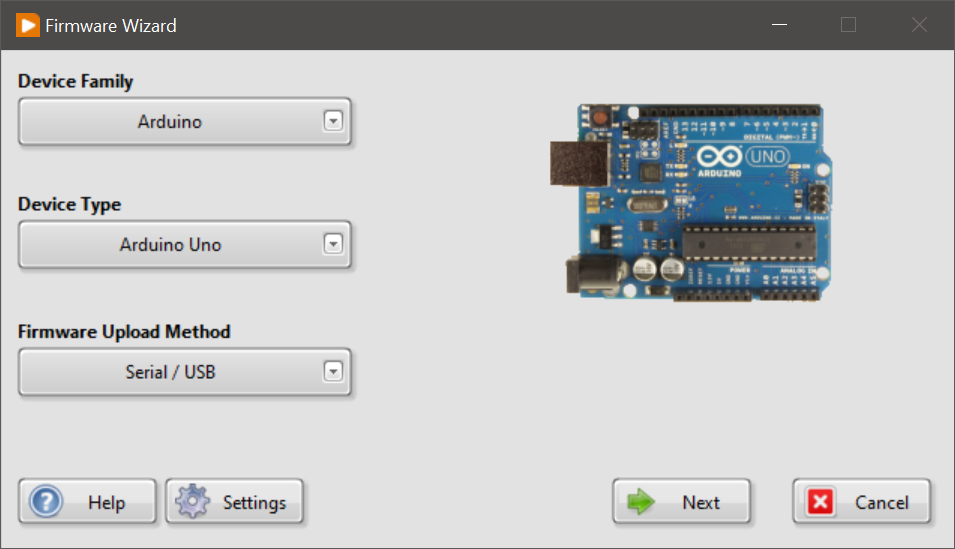
\includegraphics[width=0.75\textwidth]{FirmwareTool}
	\caption{The LiNX firmware wizard, we use this tool to make the Arduino learn $\labview$.}
	\label{FirmwareTool}
\end{figure}
Pressing next will take you to the port selection screen, make sure you select the COM port your Arduino board is connected to. If you do not see it here, make sure that you have the device plugged in and that the drivers for it is installed.\\

The last screen you should leave as is, figure \ref{FirmwareConf}, it sets the method in which the wizard flashes the microcontroller, in this case Serial/USB, and what type of firmware to install. It is possible to create your own firmware, but this beyond the scope of this book.\\
\begin{figure}
	\centering
	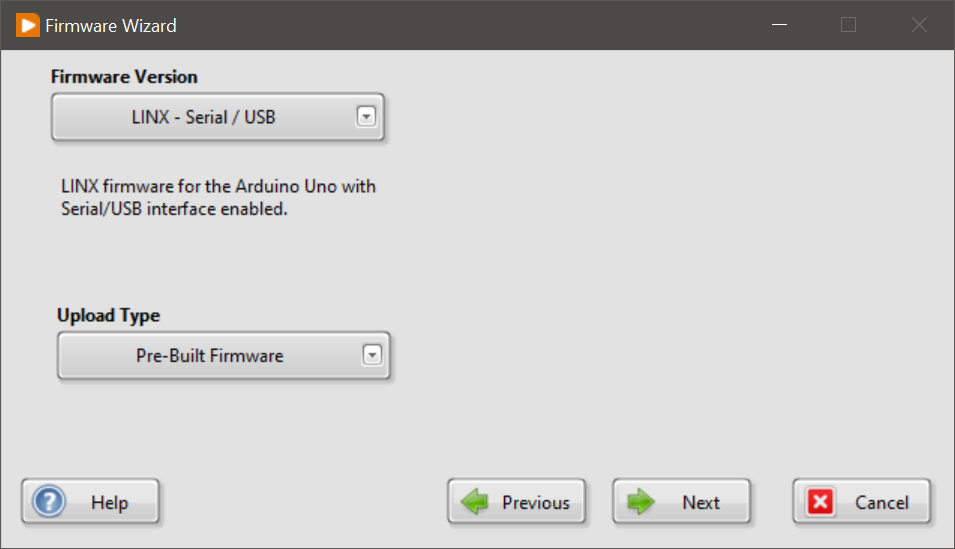
\includegraphics[width=0.75\textwidth]{FirmwarePath}
	\caption{Firmware flash settings screen, you should leave this as is.}
	\label{FirmwareConf}
\end{figure}

Once the firmware flashing is complete, a friendly window will tell you so, press the ``Launch Example'' button to test drive the new system. Figure \ref{BuiltInArduinoEg} shows the VI that opens. %TODO Add the picture please
 Here you set the COM port, like you did previously, and select the output channel to be 13. Run this VI and press the LED that says ``Click Here'', you will observe that the LED on your Arduino reflects the status of the LED in the VI. Go ahead and press it as many times as you like, you now have control over a real world object through the power of your mouse.
 
\section{Writing and Reading Ports}
We now take a small step back in time to review how Arduino code is structured. Figure \ref{ArduinoStartCode} shows the typical structure of an Arduino project. The ``setup'' block runs once, this is where \textit{you} configure all the inputs and outputs of the Arduino board and provide the code to setup a LCD display module, for example. The ``run'' loop runs continuously %TODO check naming of this loop
performing the instructions step-by-step, until the end of time, or when the power cable is unplugged.\\

Fortunately, you may use the same development patern for building code, for the Arduino, in $\labview$. There are few little extras along the way, such as opening a link to a board and managing the closing of any connections you made.\\

It is right about now where you will realise the power of $\labview$, not so much in the graphical programming style, but the amount of libraries that exist to ease the development of prototype projects.\\

\subsection{Opening a serial port to an Arduino}
Since there are multiple devices connected to your computer, and if you use a laptop those connections are internal, it is not possible to simply plug in your Arduino and expect $\labview$ to connect to your device automatically. The moment you plug in the USB cable into your computer, your operating system assigns a name to the port the new device is plugged into. It is usually "COM4" for me, but obviously your number might be different.\\

You need to provide this name to $\labview$ and tell it to open the Arduino, this is shown in figure \ref{OpenPort}. This function then gives you a resource value ``LiNX Resource''  which you will need to use communicate with the Arduino. The device name is just some description and not useful if you have only one device. The ``Error Out'' wire will hand you an error variable if something went wrong with the function.\\
\begin{figure}
	\centering
	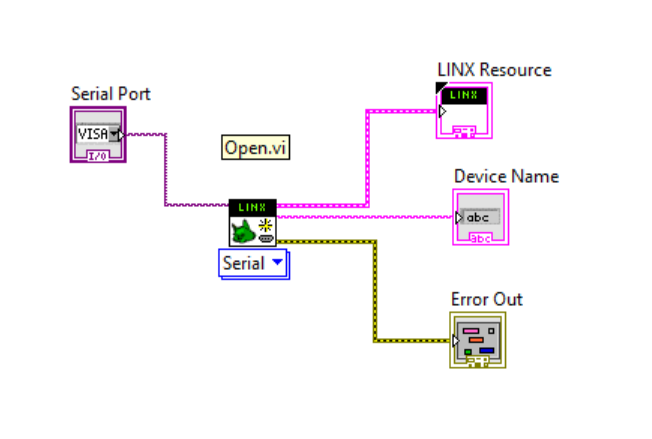
\includegraphics[width=0.70\textwidth]{ArduinoMainOpen}
	\caption{Using $\labview$ to open a port to an Arduino.}
	\label{OpenPort}
\end{figure}
\subsection{Configuring I/O}
With the Arduino now open, you can configure inputs and outputs. You have direct access to all analogue and digital outputs, however some sensors and extensions require you to open a port to initialise the device.\\

Figure \ref{OpenPorts} shows how to open a port to a servo motor and a SPI serial channel. The functions are connected in series, this means that the functions are executed one after the other.\\
\begin{figure}
	\centering
	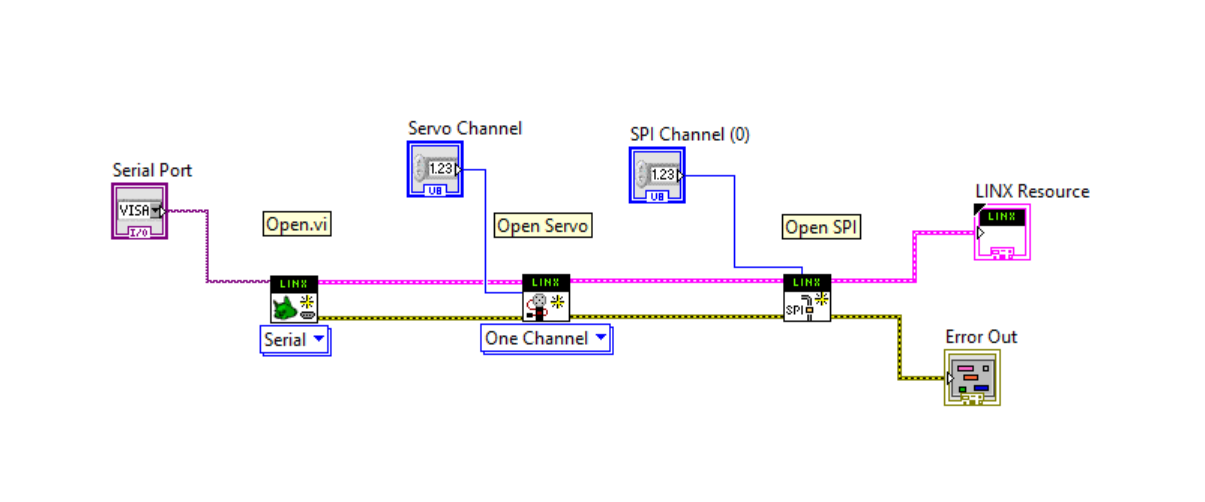
\includegraphics[width=\textwidth]{ArdOpenPorts}
	\caption{After the Arduino is connected, you can open specific devices on the Arduino.}
	\label{OpenPorts}
\end{figure}
\subsection{The main program loop} 
If there is no program loop, the program will execute once and do nothing. Most things physical process that occur in nature occur over time, quite obviously. Thus we need some way to have our little Arduino do some work for us over time.\\

Figure \ref{ProgLoopArd} shows an example of a program loop. The loop constantly checks the input called ``Pulse Width'', this value is sent to the servo motor in order to move it to the desired direction. The loop then sends the value of the shift register to an digital channel, this channel could be connected to a LED on your breadboard which would turn it on. The loop then waits one second and starts again.\\
\begin{figure}
	\centering
	\includegraphics[width=0.80\textwidth]{ArdLEDOFON}
	\caption{A simple loop turning a LED on and off, also allowing control of a servo motor.}
	\label{ProgLoopArd}
\end{figure}
\subsection{Closing all connections}
Once your program has reached the end of its life, there are some actions you will need to perform in order to shut down the Arduino safely. Back in the day, in order to shut down your computer, you had to shutdown windows and wait until a ominous message is shown on the monitor, figure \ref{Shutdown98} before you can press the power button.\\
\begin{figure}
	\centering
	
\includegraphics[width=0.80\textwidth]{Safeshutdown}
	\caption{Is it really safe though?}
	\label{Shutdown98}
\end{figure}

Although not strictly necessary, you should do the same with the Arduino. It closes the serial port properly and prevents an open port from hanging. When a port hangs, it is impossible to reopen a port from $\labview$ and you will need to do some other fancy things to get back to your beloved Arduino.\\

Figure \ref{ArdClose} shows how this simple procedure is done. It is wise to close ports to peripherals as well in case they require some special closing operations to prevent damage.
\begin{figure}
	\centering
	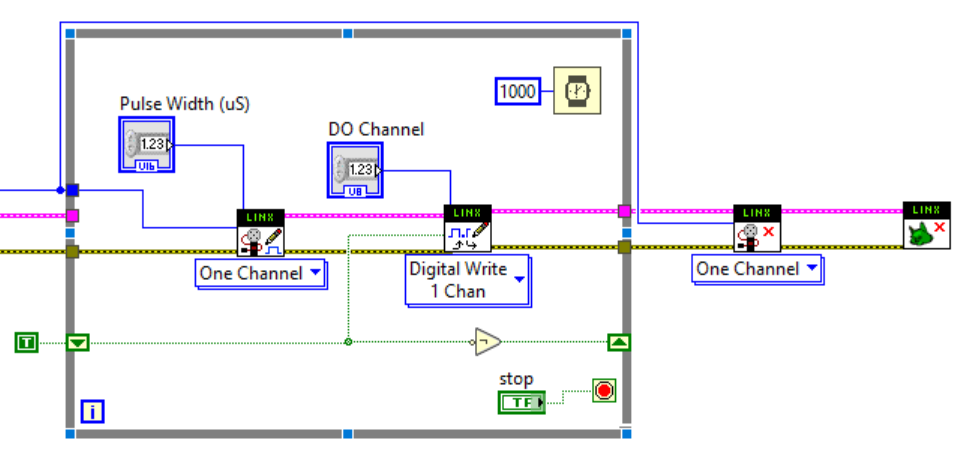
\includegraphics[width=0.80\textwidth]{ArdClose}
	\caption{Final closing operations before the program stops.}
	\label{ArdClose}
\end{figure}
\section{Quite Advanced Projects}
\begin{enumerate}
	\item \textbf{Build an access control system:}\\
	You need to build an access control system for your lab. Recently a very expensive diamond anvil has been stolen from the lab and your supervisor needs you to make sure that people who don't belong in the lab stay outside. \\
	
	Tier 1 $\left(40\%\right)$; Design and implement a program which allows the user to press a single button to open the door to the restricted area. The door should only open if the password given is correct. The program needs to tell the user if the password is incorrect. When you type the password, the box should not show what is being typed, instead you should see $\bullet\bullet\bullet\bullet$. The program should lock the door again after some time has passed so that it is not left open, however the door can't be locked if it is not closed so an alarm should sound if the door is left open for too long.\\
	
	 Tier 2 $\left(30\%\right)$; With the above program in place, adapt it to use an Arduino to light up some LEDs to show the status of the lock, for example, green for open and red for closed. Build a circuit to create a buzzer, adapt your program to make the Arduino sound an alarm if the door is left open for too long. Using an LCD screen with $\labview$ is easy, build an LCD module into your system which says if the door is open, closed and or locked.\\
	 
	  Tier 3 $\left(20\%\right)$; If you enter the lab and the door closes. You will need to enter the password again to open the door. Add the ability to press a button from inside the lab to override the program to open the door. Up to now you are still just pretending that you are locking a door, use your knowledge from last semester to include a solenoid into your design.\\
	  
	  Tier 3 $\left(10\%\right)$; Finally, you have access to an RFID card reader, build a program in $\labview$ to use this facility to open the lock on the door.\\
	  
	  \item \textbf{Build a Morse code generator:}\\
	  You have seen previously how to convert a string into a series of bytes, use what you have learned to create a Morse code generator that will flash an LED and sound a buzzer.\\
	  
	  Tier 1 $\left(40\%\right)$ Your program should have a user input their name, telephone number and their message to send. The program should not allow long messages to be sent. The program should then send a Morse code message (via a on-screen light). Essentially you will need to convert every byte into a pattern corresponding to Morse code.\\
	  
	  Tier 2 $\left(20\%\right)$ Build a cryptographic system into your program so that the user can send a encrypted message using your program.\\
	  
	  Tier 3 $\left(30\%\right)$ Connect the program you have built to an Arduino so that you can light up an LED and beep out the Morse code with a buzzer. You should also connect an LCD module so that it prints out your message in a way that is pleasing to you, more marks for interesting printing methods.\\
	  
	  Tier 4 $\left(10\%\right)$ Add the ability to have the user press a button to key Morse code into your program and have the program convert the code into text.\\
\end{enumerate}